\clearpage

\section{$D^0$ Reconstruction}

$D^{0}$ and $\bar{D^{0}}$ are reconstructed through the typically hadronic channel $K^{\mp}\pi^{\pm}$ using the topological method. In the following we will describe the daughter selection, the geometry cuts and how they are obtained through the TMVA tuning. We will show the $D^0$ signals for different $p_T$ bins. We will also discuss some related topics: the mixed event to reconstruct the combinatorial background, and the correlated background source shown as a `bump' at invariant mass lower than the $D^0$. 

\subsection{Daughter Selection}
\label{daughterSelection}
$D^0$ have a lifetime of $c\tau\sim123 \upmu$m. Thus the global tracks for daughter tracks are used in this analysis. The transverse momentum are required to $\geq$ 0.3 GeV/$c$ to ensure that the track can pass through the TPC and have less HFT miss matching, the number of hit points (nHits) along the track is $\geq$ 20 (of a maximum of 45) to ensure good momentum resolution.

The pion and kaon tracks are identified by combining Time Projection Chamber (TPC) and Time Of Flight detector (TOF). The TPC provides particle identification utilizing the energy loss information $dE/dx$, different particle species with the same momentum may have different $dE/dx$. In additional, different particle species with the same momentum have different velocities, thus the TOF can be used to identify different particle species in the $dE/dx$ crossover regions by precise velocity information ($1/\beta$ = $ct/l$). The normalized $dE/dx$, $n\sigma_x$ (x = $\pi$, K, p, e etc.), defined in Eq.~\ref{nsigma}, instead of $dE/dx$ is used in this analysis. Where $\langle{dE/dx}\rangle_{measured}$ and $\langle{dE/dx}\rangle_{x}$ represent measured and theoretical $dE/dx$, and $R$ is the STAR TPC $dE/dx$ resolution (typically $\sim$8\%). The $n\sigma_x$ should be close to a standard Gaussian distribution for each corresponding particle species (mean $=$ 0, $\sigma = $ 1).
\begin{equation}
  n\sigma_x = \frac{1}{R}log\frac{\langle{dE/dx}\rangle_{measured}}{\langle{dE/dx}\rangle_{x}}
\label{nsigma}
\end{equation}

Fig.~\ref{fig:tpcPID} shows the TPC energy loss dE/dx information versus momentum achieved from Run14 Au+Au 200GeV, there are several clear bands for different particle species such as $\pi$, K, p and e. 

Fig.~\ref{fig:tofPID} shows the TOF 1/Beta information versus momentum achieved from Run14 Au+Au 200GeV, also there are several clear bands for different particle species such as $\pi$, K, p . 

\begin{figure}[htbp]
\centering
\includegraphics[keepaspectratio,width=0.8\textwidth]{figure/Run14_D0HFT/Run14_AuAu_dEdx_PR_copy.png}
\caption{TPC dE/dx versus charge$\times$momentum achieved from Run14 Au+Au 200GeV.}
 \label{fig:tpcPID}
\end{figure}

\begin{figure}[htbp]
\centering
\includegraphics[keepaspectratio,width=0.8\textwidth]{figure/Run14_D0HFT/Run14_AuAu_tofBeta_PR.png}
\caption{TOF 1/Beta versus momentum achieved from Run14 Au+Au 200GeV.}
 \label{fig:tofPID}
\end{figure}

In summary, next list all the related track selections for $D^0$ daughters including track quality cut and particle identification cut.
\begin{itemize}
\item global tracks
\item $p_{T}$ > 0.3 GeV/$c$ (next plots are based on 0.3 GeV cut, but the final result central value was from 0.6 GeV cut, same as $D^0$ v2 analysis)
% \item $p_{T}$ > 0.6 GeV/$c$
\item $|\eta| < 1$
\item $nHitsFit \ge 20$, in TPC
\item at least one hit in every layer of PXL and IST
\end{itemize}

pion PID:
\begin{itemize}
  \item $|n\sigma_{\pi}| < 3.0 $, based on TPC dE/dx
  \item If TOF is avaliable (hybrid PID):  $|\frac{1}{\beta}-\frac{1}{\beta_{exp}}|<0.03$
\end{itemize}

kaon PID:
\begin{itemize}
  \item $|n\sigma_{K}| < 2.0 $, based on TPC dE/dx
  \item If TOF is avaliable (hybrid PID):  $|\frac{1}{\beta}-\frac{1}{\beta_{exp}}|<0.03$
\end{itemize}


\subsection{Topological Cut Optimization}

The secondary vertex is reconstructed with selected kaon and pion global tracks. In this analysis, the middle point on the Distance of the Closest Approach (DCA) between two daughter tracks is considered as the secondary decay vertex of the candidate $D^0$. As shown in Fig.~\ref{fig:D0cartoon}, 5 geometrical variables are chosen to select $D^0$ and reject combinatorial background, which is dominated by a pair of tracks directly from the primary vertex: decay length (the distance between the decay vertex and Primary Vertex PV), DCA between the 2 daughters, DCA between the reconstructed $D^0$ flying path and PV, DCA between the $\pi$ track and PV, and DCA between the $K$ track and PV. The cuts on these variables are optimized by the Toolkit for Multivariate Data Analysis (TMVA) package. They change according to the $D^0$ candidate $p_T$ in order to have the best significance in all the covered $p_T$ range. Additionally there is a $cos(\theta) > 0$ cut to make sure the decay vertex with respect to the primary vertex is roughly in the same direction as the momentum.

\begin{figure}[htbp]
\centering
\includegraphics[keepaspectratio,width=0.6\textwidth]{figure/Run14_D0HFT/D0cartoon.png}
\caption{The topology of a $D^0$ decaying to a kaon and a pion.}
 \label{fig:D0cartoon}
\end{figure}

The TMVA need signal and background sample input for training. The signal sample is obtained from a toy fast-simulation and the background sample is from real data like sign pairs in $D^0$ mass window and unlike sign pairs in side bands range. 

Fig.~\ref{fig:variables} shows distributions of the 5 geometry variables for signal (blue) and background (red) plotted by the TMVA, for $p_T$ between 2 and 3 GeV/$c$.

\begin{figure}[htbp]
\centering
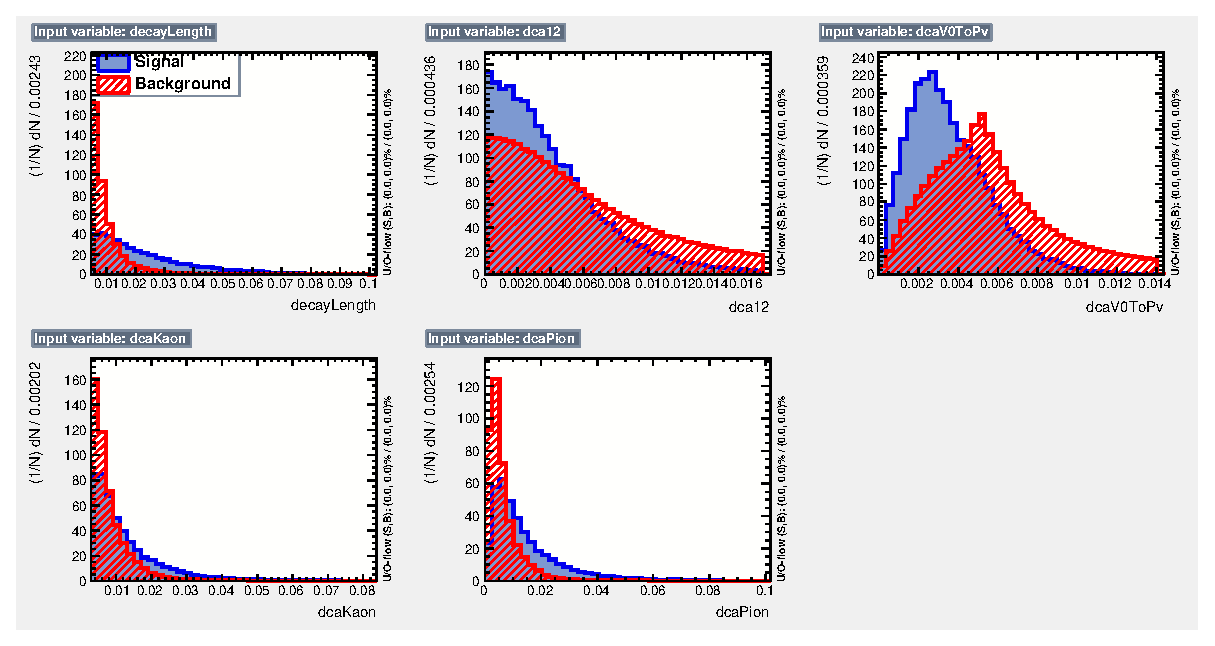
\includegraphics[keepaspectratio,width=1.0\textwidth]{figure/Run14_D0HFT/variables_id_c1.eps}
\caption{Distributions of the 5 geometry variables for signal (blue) and background (red).}
\label{fig:variables}
\end{figure}

The `cuts' option of TMVA is used to tune $D^0$ cuts. This option randomly sample different cut sets in the variable space, calculate signal and background efficiency for each cut set. Then one cut set with lowest background efficiency at certain signal efficiency. We can then pick the cut set with the best significance according to the signal and background yield corresponding to the whole data set. Fig.~\ref{fig:effPass4} shows the lowest background efficiency, significance and so on vs. signal efficiency for $p_T$ between 2 and 3 GeV/$c$. We can see that as cuts get tighter, signal and background efficiency both decrease, but background efficiency decreases much faster.

\begin{figure}[htbp]
\centering
\includegraphics[keepaspectratio,width=0.5\textwidth,angle=0]{figure/Run14_D0HFT/effPass4.pdf}
\caption{Signal efficiency, lowest background efficiency, significance and so on vs. signal efficiency.}
\label{fig:effPass4}
\end{figure}

\begin{table}[htp]
  \centering
  \caption{Standard geometrical cuts for different $D^0$ $p_T$.}
  \label{geometryCuts}
  \begin{center}
    \begin{tabular}{l|l|l|l|l|l}
      % \Xhline{1.6pt}
      $D^0$ $p_T$ (GeV/$c$) & 0-1 & 1-2 & 2-3 & 3-5 & 5-10\\ \hline
      decay length (${\upmu}m$) $>$ & 145 & 181 & 212 & 247 & 259\\ \hline
      DCA between 2 daughters (${\upmu}m$) $<$ & 84 & 66 & 57 & 50 & 60\\ \hline
      DCA between $D^0$ and PV (${\upmu}m$) $<$ & 61 & 49 & 38 & 38 & 40\\ \hline
      DCA between $\pi$ and PV (${\upmu}m$) $>$ & 110 & 111 & 86 & 81 & 62\\ \hline
      DCA between $K$ and PV (${\upmu}m$) $>$ & 103 & 91 & 95 & 79 & 58\\ \hline
      % \Xhline{1.6pt}
    \end{tabular}
  \end{center}
\end{table}

\begin{table}[htp]
  \centering
  \caption{Tight geometrical cuts for different $D^0$ $p_T$.}
  \label{geometryCutsTight}
  \begin{center}
    \begin{tabular}{l|l|l|l|l|l}
      % \Xhline{1.6pt}
      $D^0$ $p_T$ (GeV/$c$) & 0-1 & 1-2 & 2-3 & 3-5 & 5-10\\ \hline
      decay length (${\upmu}m$) $>$ & 144 & 204 & 242 & 245 & 300\\\hline
      DCA between 2 daughters (${\upmu}m$) $<$ & 69 & 48 & 44 & 49 & 47\\ \hline
      DCA between $D^0$ and PV (${\upmu}m$) $<$ & 44 & 36 & 31 & 26 & 32\\ \hline
      DCA between $\pi$ and PV (${\upmu}m$) $>$ & 120 & 102 & 118 & 109 & 96\\ \hline
      DCA between $K$ and PV (${\upmu}m$) $>$ & 119 & 110 & 109 & 106 & 80\\ \hline
      % \Xhline{1.6pt}
    \end{tabular}
  \end{center}
\end{table}


\begin{table}[htp]
  \centering
  \caption{Loose geometrical cuts for different $D^0$ $p_T$.}
  \label{geometryCutsLoose}
  \begin{center}
    \begin{tabular}{l|l|l|l|l|l}
      % \Xhline{1.6pt}
      $D^0$ $p_T$ (GeV/$c$) & 0-1 & 1-2 & 2-3 & 3-5 & 5-10\\ \hline
      decay length (${\upmu}m$) $>$ & 110 & 168 & 187 & 199 & 180\\ \hline
      DCA between 2 daughters (${\upmu}m$) $<$ & 77 & 78 & 74 & 68 & 66\\ \hline
      DCA between $D^0$ and PV (${\upmu}m$) $<$ & 72 & 53 & 47 & 42 & 62\\ \hline
      DCA between $\pi$ and PV (${\upmu}m$) $>$ & 92 & 78 & 86 & 65 & 47\\ \hline
      DCA between $K$ and PV (${\upmu}m$) $>$ & 105 & 68 & 80 & 66 & 41\\ \hline
      % \Xhline{1.6pt}
    \end{tabular}
  \end{center}
\end{table}

The result of the geometry cuts tuned for best significance are shown in Table \ref{geometryCuts}. These are the standard cuts used in the $D^0$ reconstruction to calculate the spectra central value.

For $D^0$ estimation, another 2 sets of geometry cuts are tuned with TMVA, with 50\% and 150\% signal efficiency relative to the standard cuts. They do not give the overall best $D^0$ significance, but for the certain signal efficiency, they are still the cuts with the lowest background efficiency and best $D^0$ significance. With 50\% and 150\% signal efficiency relative to the standard cuts, their significance is still about 80\% of the standard cuts with the overall best significance. These 2 cuts sets are listed in Table \ref{geometryCutsTight} and \ref{geometryCutsLoose}.

For more details can be found in the $D^0$ $v_2$ technicl note, basically we use the same cuts for spectra analysis and $v_2$ analysis.

\subsection{Mixed Event Background}

To construct the mixed event background it is important to combine events with some degree of similarity, such as events are classified according to the position of the primary vertex (PV) along the beam-line, the centrality class and the orientation of the event plane. Ten bins of equal width were used for both the event plane ($\Psi\in[-\pi,\pi]$) and the position of the primary vertex($V_z\in[-6,6]$), as well as nine centrality classes between 0-80\%, for a total of 900 event `categories'.

Table \ref{eventBuf} summarizes the important information saved for the event mixing:

\begin{table}[htp]
\centering
\caption{Summary of information saved for the event mixing}
\label{eventBuf}
\begin{tabular}{ l | l  }
\toprule[1.6pt]
StMixerTrack & StMixerEvent \\
\midrule[1.2pt]
Origin & PV Origin \\
\\
Momentum & Magnetic Field \\
\\
Q-Vector & Event Plane \\
\\
Track information & Array of mixer tracks \\
\\
  &Array of indices to identified pions \\
\\
  & Array of indices to identified kaons \\
\\
\bottomrule[1.6pt]
\end{tabular}
\end{table}

Fig.~\ref{fig:mixedEvent_pt1_2} and Fig.~\ref{fig:mixedEvent_pt4_5} show the invariant mass distribution for the foreground and two different uncorrelated backgrounds: same event like-sign and mixed event unlike-sign in two $p_T$ bins include 1-2 GeV/$c$ and 4-5 GeV/$c$. The mixed event backgrounds have been scaled to the foreground using the integration range $m_{K\pi}\in[1.6,2.1]$ GeV/$c^{2}$.

\begin{figure}[htbp]
\centering
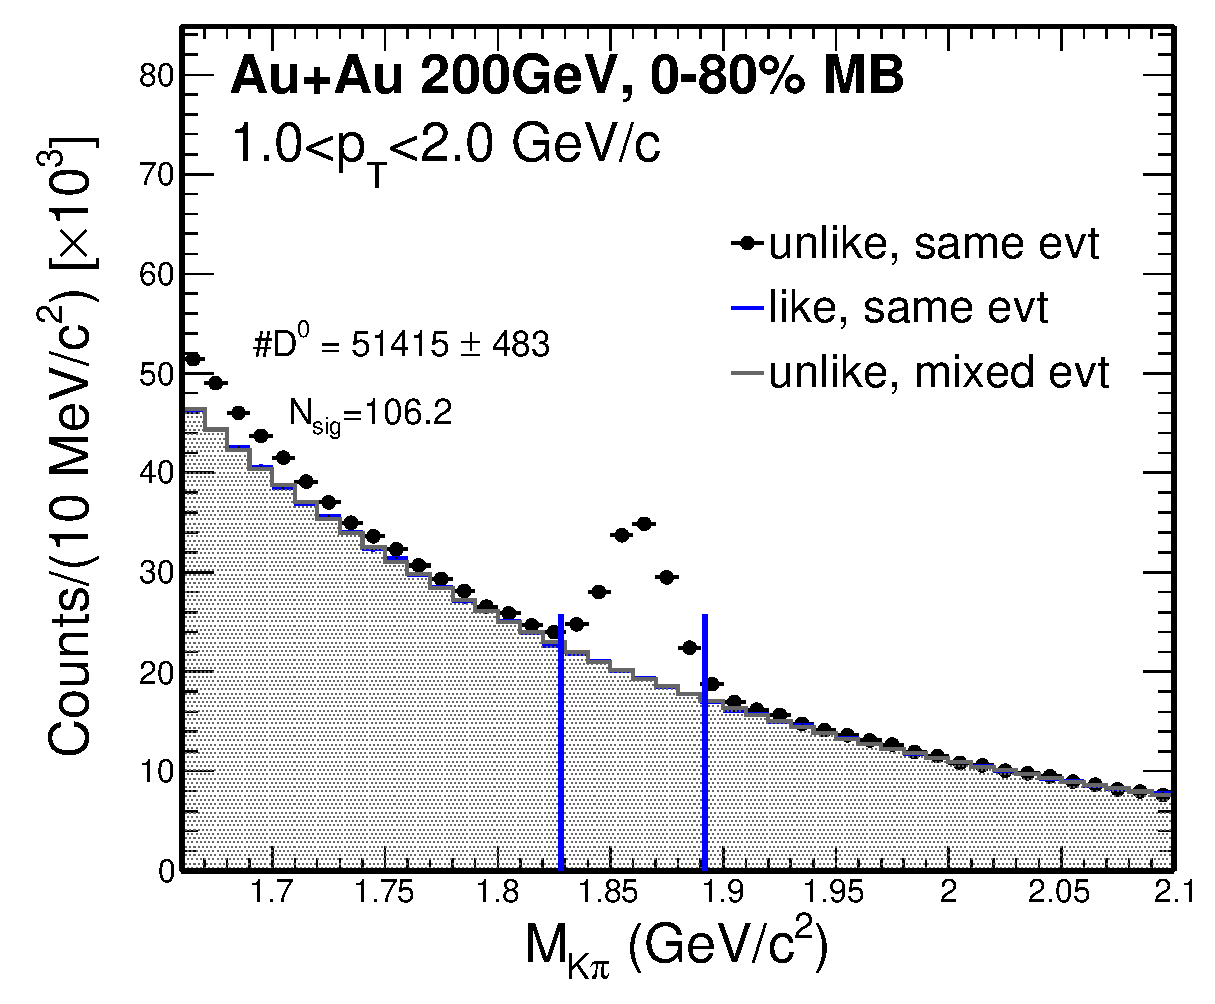
\includegraphics[keepaspectratio,width=0.6\textwidth]{figure/Run14_D0HFT/Mixed_cent_1_9_pt_1_2.eps}
\caption{Invariant mass distribution for foreground and two descriptions of combinatorial background in 1 < $p_T$ < 2 GeV/$c$.}
\label{fig:mixedEvent_pt1_2}
\end{figure}

\begin{figure}[htbp]
\centering
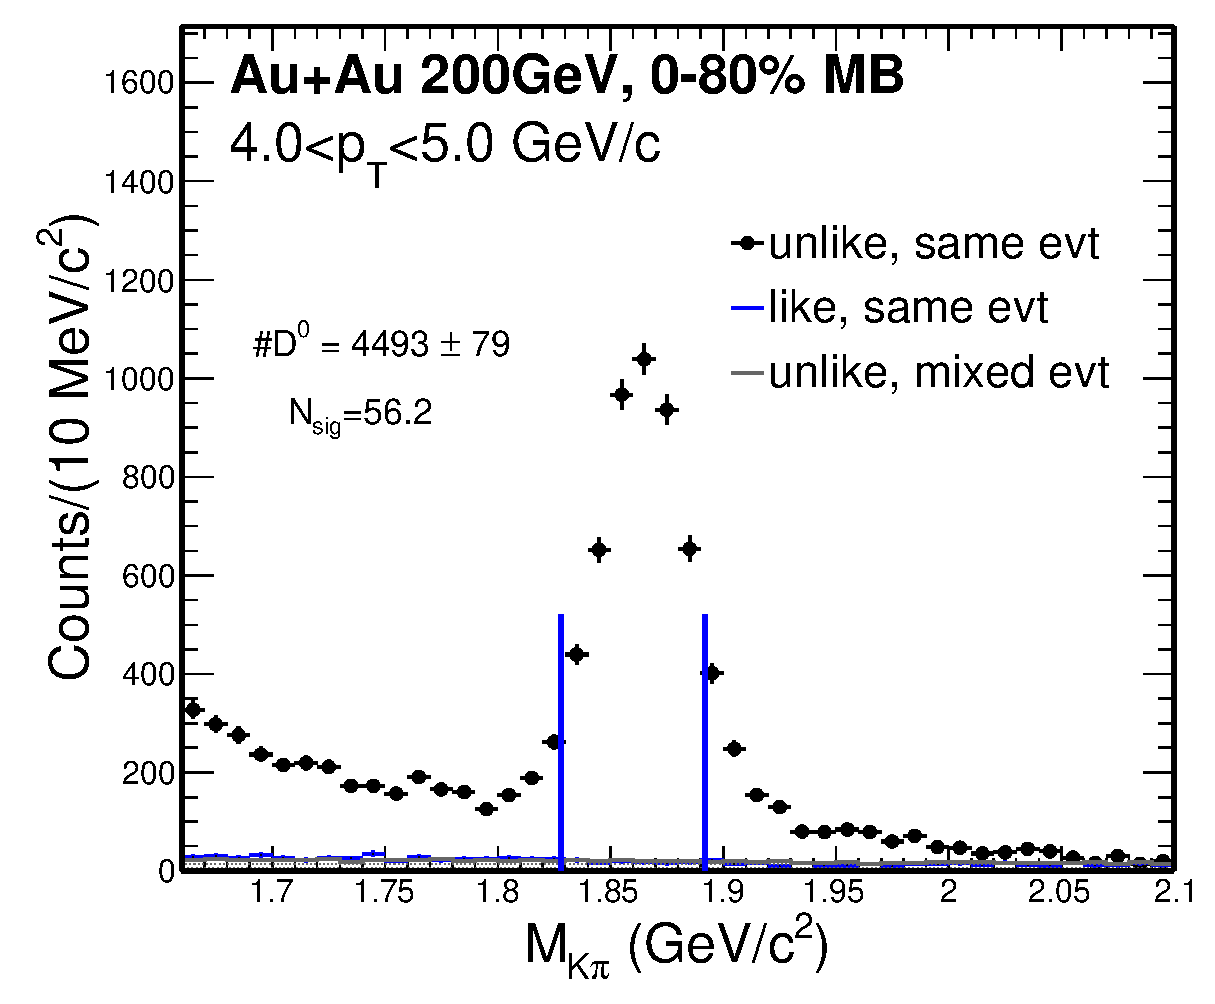
\includegraphics[keepaspectratio,width=0.6\textwidth]{figure/Run14_D0HFT/Mixed_cent_1_9_pt_4_5.eps}
\caption{Invariant mass distribution for foreground and two descriptions of combinatorial background in 4 < $p_T$ < 5 GeV/$c$.}
\label{fig:mixedEvent_pt4_5}
\end{figure}

There is good agreement between the two descriptions of the combinatorial background and they appear to provide an adequate description in the vicinity of the $D^0$ signal and the mixed event backgrounds have improved statistical precision.

It is interesting to observe the presence of an `excess' in the foreground, relative to all of the background curves, below roughly 1.75 GeV/$c^2$.  This so called bump was investigated using the Data Driven Fast Simulator, and will be covered briefly in the following section.

\subsection{Correlated background `bump' for $D^0$ meson}

The contributions to the invariant mass spectrum from the following $D^0$ and $D^\pm$ decays were included in a qualitative study of the correlated background: 

\begin{itemize}
\item $D^0 \rightarrow K^-\pi^+$ (B.R. 0.039)
\item $D^0 \rightarrow  K^-\pi^+\pi^0$ (B.R. 0.011)
\item $D^0 \rightarrow  K^-\rho^+ \rightarrow K^-\pi^+\pi^0$ (B.R. 0.108)
\item $D^0 \rightarrow  K^{*-}\pi^+\rightarrow K^-\pi^+\pi^0$ (B.R. 0.007)
\item $D^+ \rightarrow  K^-\pi^+\pi^+$ (B.R. 0.073 $\times$ 0.415)
\end{itemize}

The charm fragmentation ratio used is the following from ZEUS Collaboration (arXiv:hep-ex/0508019 - Table 4):

\begin{itemize}
\item f($c \rightarrow D^+$) = 0.217 
\item f($c \rightarrow D^0$) = 0.523 
\item f($c \rightarrow D^+_s$) = 0.095
\item f($c \rightarrow \Lambda^+_c$) = 0.144
\item f($c \rightarrow D^{*+}$) = 0.200
\end{itemize}

\begin{figure}[htbp]
\centering
\includegraphics[keepaspectratio,width=0.7\textwidth,angle=0]{figure/Run14_D0HFT/D0Bump_without_topo.pdf}
\caption{Simulated contribution to the invariant mass spectrum from cocktail without topological cut}
\label{fig:cocktail1}
\end{figure}

\begin{figure}[htbp]
\centering
\includegraphics[keepaspectratio,width=0.7\textwidth,angle=0]{figure/Run14_D0HFT/D0Bump_with_topo.pdf}
\caption{Simulated contribution to the invariant mass spectrum from cocktail with topological cut}
\label{fig:cocktail2}
\end{figure}

Fig.~\ref{fig:cocktail1} and Fig.~\ref{fig:cocktail2} show the invariant mass spectrum obtained from the cocktail after scaling by the branching ratio for different decays as well as the fragmentation ratio for the different charmed meson species.

The spectrum is shown before and after the $D^0\rightarrow K\pi$ topological cuts have been applied. It is clear that the contributions from correlated background can, at least in part, account for the enhancement observed below roughly 1.7 GeV/$c^2$.

The cocktail simulation was then scaled by fitting the amplitude of the $D^0$ peak obtained from fast simulator to the signal observed in data, and the cocktail was then added to the mixed event background. Fig.~\ref{fig:bump1} and Fig.~\ref{fig:bump2} shows a comparison between the invariant mass distribution obtained from data and the spectrum obtained by combining the mixed event background and the results from the data-driven Fast-Simulator.

\begin{figure}[htbp]
\centering
\includegraphics[keepaspectratio,width=0.7\textwidth]{figure/Run14_D0HFT/D0_FG_EvMxBg_coktail_2040_2_pT_3.png}
\caption{Comparison of $K\pi$ invariant mass distribution for unlike-sign (US) foreground, like-sign combinatorial background, unlike-sign (US) mixed events combinatorial background, and unlike-sign (US) mixed events combinatorial background + toy montecarlo cocktail for correlated background, for 2 < $p_T$ < 3 GeV/$c$.}
\label{fig:bump1}
\end{figure}

\begin{figure}[htbp]
\centering
\includegraphics[keepaspectratio,width=0.7\textwidth]{figure/Run14_D0HFT/D0_FG_EvMcBg_cocktail_2040_3_pT_10.png}
\caption{Similar Comparison of $K\pi$ invariant mass distribution as Fig.~\ref{fig:bump1}, for 3 < $p_T$ < 10 GeV/$c$.}
\label{fig:bump2}
\end{figure}

The inclusion of correlated background sources can qualitatively describe the foreground observed, reproducing the location of the bump structure albeit underestimating the degree of enhancement itself. Furthermore, there is likely a finite contribution to the observed bump originating from jet correlations which should be included to improve on the description of the background.

It should also be noted that the studies presented here were done with an early version of the fast simulator which only included the $p_T$ and centrality dependence of sampled distributions, revisiting the studies with more differential distributions should improve on these results.

Nonetheless, the results provide confidence in a qualitative understanding on the sources of the correlated background and, what is more, suggest that the contribution from these source in the $D^0$ signal range is dominated by double mis-PID, and is nearly negligible as shown in the following sub-section.

% For the more details of the mixed-event backgrounds and the `bump' structures in the foreground, they also can be found in the $v_2$ analysis note.